\section{Code Generation Pipeline}


\subsection{Generation Architecture}

\begin{figure}[h]
\centering
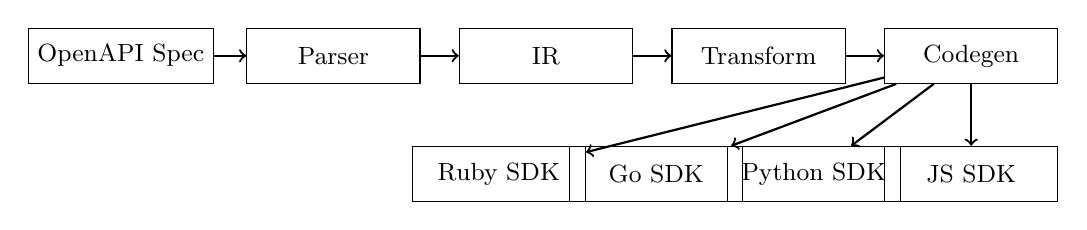
\begin{tikzpicture}[
    node distance=1.5cm,
    box/.style={rectangle, draw, minimum width=2.2cm, minimum height=0.7cm, font=\small},
    arrow/.style={->, thick}
]
    \node[box] (spec) {OpenAPI Spec};
    \node[box, right of=spec, xshift=1.2cm] (parse) {Parser};
    \node[box, right of=parse, xshift=1.2cm] (ir) {IR};
    \node[box, right of=ir, xshift=1.2cm] (transform) {Transform};
    \node[box, right of=transform, xshift=1.2cm] (codegen) {Codegen};

    \node[box, below of=codegen, yshift=0cm] (js) {JS SDK};
    \node[box, left of=js, xshift=-0.5cm] (py) {Python SDK};
    \node[box, left of=py, xshift=-0.5cm] (go) {Go SDK};
    \node[box, left of=go, xshift=-0.5cm] (rb) {Ruby SDK};

    \draw[arrow] (spec) -- (parse);
    \draw[arrow] (parse) -- (ir);
    \draw[arrow] (ir) -- (transform);
    \draw[arrow] (transform) -- (codegen);
    \draw[arrow] (codegen) -- (js);
    \draw[arrow] (codegen) -- (py);
    \draw[arrow] (codegen) -- (go);
    \draw[arrow] (codegen) -- (rb);
\end{tikzpicture}
\caption{Code generation pipeline}
\end{figure}

\subsection{Intermediate Representation}

\begin{definition}[SDK IR]
The intermediate representation $I$ comprises:
\begin{itemize}
    \item $\mathcal{R}$: Set of resources with operations
    \item $\mathcal{M}$: Set of models (request/response types)
    \item $\mathcal{E}$: Set of error types
    \item $\mathcal{C}$: Configuration options
\end{itemize}
\end{definition}

\begin{lstlisting}[caption=IR Structure]
interface Resource {
  name: string;
  path: string;
  operations: Operation[];
  nestedResources: Resource[];
}

interface Operation {
  name: string;
  httpMethod: HttpMethod;
  path: string;
  parameters: Parameter[];
  requestBody?: Model;
  responseBody: Model;
  errors: Error[];
}

interface Model {
  name: string;
  properties: Property[];
  required: string[];
}
\end{lstlisting}

\subsection{Language Transformations}

Each target language applies transformations:

\begin{algorithm}
\caption{Language-Specific Transformation}
\begin{algorithmic}[1]
\Function{Transform}{$ir$, $language$}
    \State $transformed \gets copy(ir)$
    \For{$model \in transformed.models$}
        \State $model.name \gets$ \Call{TransformName}{$model.name$, $language$}
        \For{$prop \in model.properties$}
            \State $prop.name \gets$ \Call{TransformProperty}{$prop.name$, $language$}
            \State $prop.type \gets$ \Call{MapType}{$prop.type$, $language$}
        \EndFor
    \EndFor
    \For{$resource \in transformed.resources$}
        \For{$op \in resource.operations$}
            \State $op.name \gets$ \Call{TransformMethod}{$op.name$, $language$}
        \EndFor
    \EndFor
    \State \Return $transformed$
\EndFunction
\end{algorithmic}
\end{algorithm}

\subsubsection{Naming Conventions}

\begin{table}[h]
\centering
\caption{Naming Convention Transformations}
\begin{tabular}{lllll}
\toprule
\textbf{Concept} & \textbf{JavaScript} & \textbf{Python} & \textbf{Go} & \textbf{Ruby} \\
\midrule
Class & PascalCase & PascalCase & PascalCase & PascalCase \\
Method & camelCase & snake\_case & PascalCase & snake\_case \\
Property & camelCase & snake\_case & PascalCase & snake\_case \\
Constant & UPPER\_CASE & UPPER\_CASE & PascalCase & UPPER\_CASE \\
\bottomrule
\end{tabular}
\end{table}

\subsubsection{Type Mapping}

\begin{table}[h]
\centering
\caption{Type Mappings}
\begin{tabular}{lllll}
\toprule
\textbf{OpenAPI} & \textbf{JavaScript} & \textbf{Python} & \textbf{Go} & \textbf{Ruby} \\
\midrule
string & string & str & string & String \\
integer & number & int & int64 & Integer \\
number & number & float & float64 & Float \\
boolean & boolean & bool & bool & Boolean \\
array & T[] & List[T] & []T & Array \\
object & Record & Dict & map & Hash \\
\bottomrule
\end{tabular}
\end{table}

